\chapter{Results}\label{cha:Research}
%

% Ska följa som ett naturligt komplement till huvuddelen

In this chapter, the results are presented, so that in the next chapter, these results are analysed. \todo{Flytta Insights som besvarar en Research Question till Discussion, och hänvisa till iteration. I Resultat vill vi bara ha Resultat, ej svar på forskningsfrågor, så spara svar på forskningsfrågor tills Diskussion.}

%\section{Example}\label{sec:research:history}
%
Liksom \citep{Duck:2005} har vi kommit fram till att glass smakar bäst på sommaren \citep{Khalil02NonlinearSystemsBook}.

\marginpar{Kommer att tänka på en liten anekdot\ldots}

\Warning[TODO]{Ta bort den löjliga anekdoten!}

\begin{figure}[tbp]
  \centering
  \subfloat[Alldeles för tidigt.][\label{fig:times:very-early}Det här är väl tidigt — din glass hinner smälta innan ditt sällskap dyker upp.]{\includegraphics[page=1]{clocks}}
  \qquad
  \subfloat[Med marginal.][\label{fig:times:early}Kiosken stänger snart, men inte nu — perfekt!]{\includegraphics[page=2]{clocks}}
  \\
  \subfloat[I grevens tid.][\label{fig:times:on-time}Precis i tid — du får in ett finger i luckan just när kiosken ska stänga.  Han som jobbar blir sur, och det blir smolk i bägaren.]{\includegraphics[page=3]{clocks}}
  \qquad
  \subfloat[Försent.][\label{fig:times:late}Du är sen — kiosken är stängd.]{\includegraphics[page=4]{clocks}}
  \caption{\label{fig:times}%
    Illustration av \emph{subfloats}.  Den så kallade \emph{bounding box}en visas i \protect\subref{fig:times:late}.  Lägg märke till att bounding boxen har satts så att alla bilder har samma storlek, med enhetlig placering av själva innehållet i förhållande till bounding boxen.  Antag att du ska träffa en kompis för att äta glass just när kiosken stänger för dagen vid 08:30.  När dyker du upp?}
\end{figure}

\section{Developed Application}

  In figure~\ref{fig:iteration-map} the end results of the app from iteration 1, 2, 3 and 4 are shown. The final app works on web or as an app, online or offline, on all of YoungDrive's Android and iOS devices. The app is fast to use, the back button on the phone can be used to go to the previous view, and the font size and images are consistent for each screen (which was not the case iteration 1-3, see figure). The goal was to provide a great learning experience, with a strong YoungDrive feel (embracing the values of fun, plus using the YoungDrive logo and colors)

  \begin{figure}[h]
    \centering
    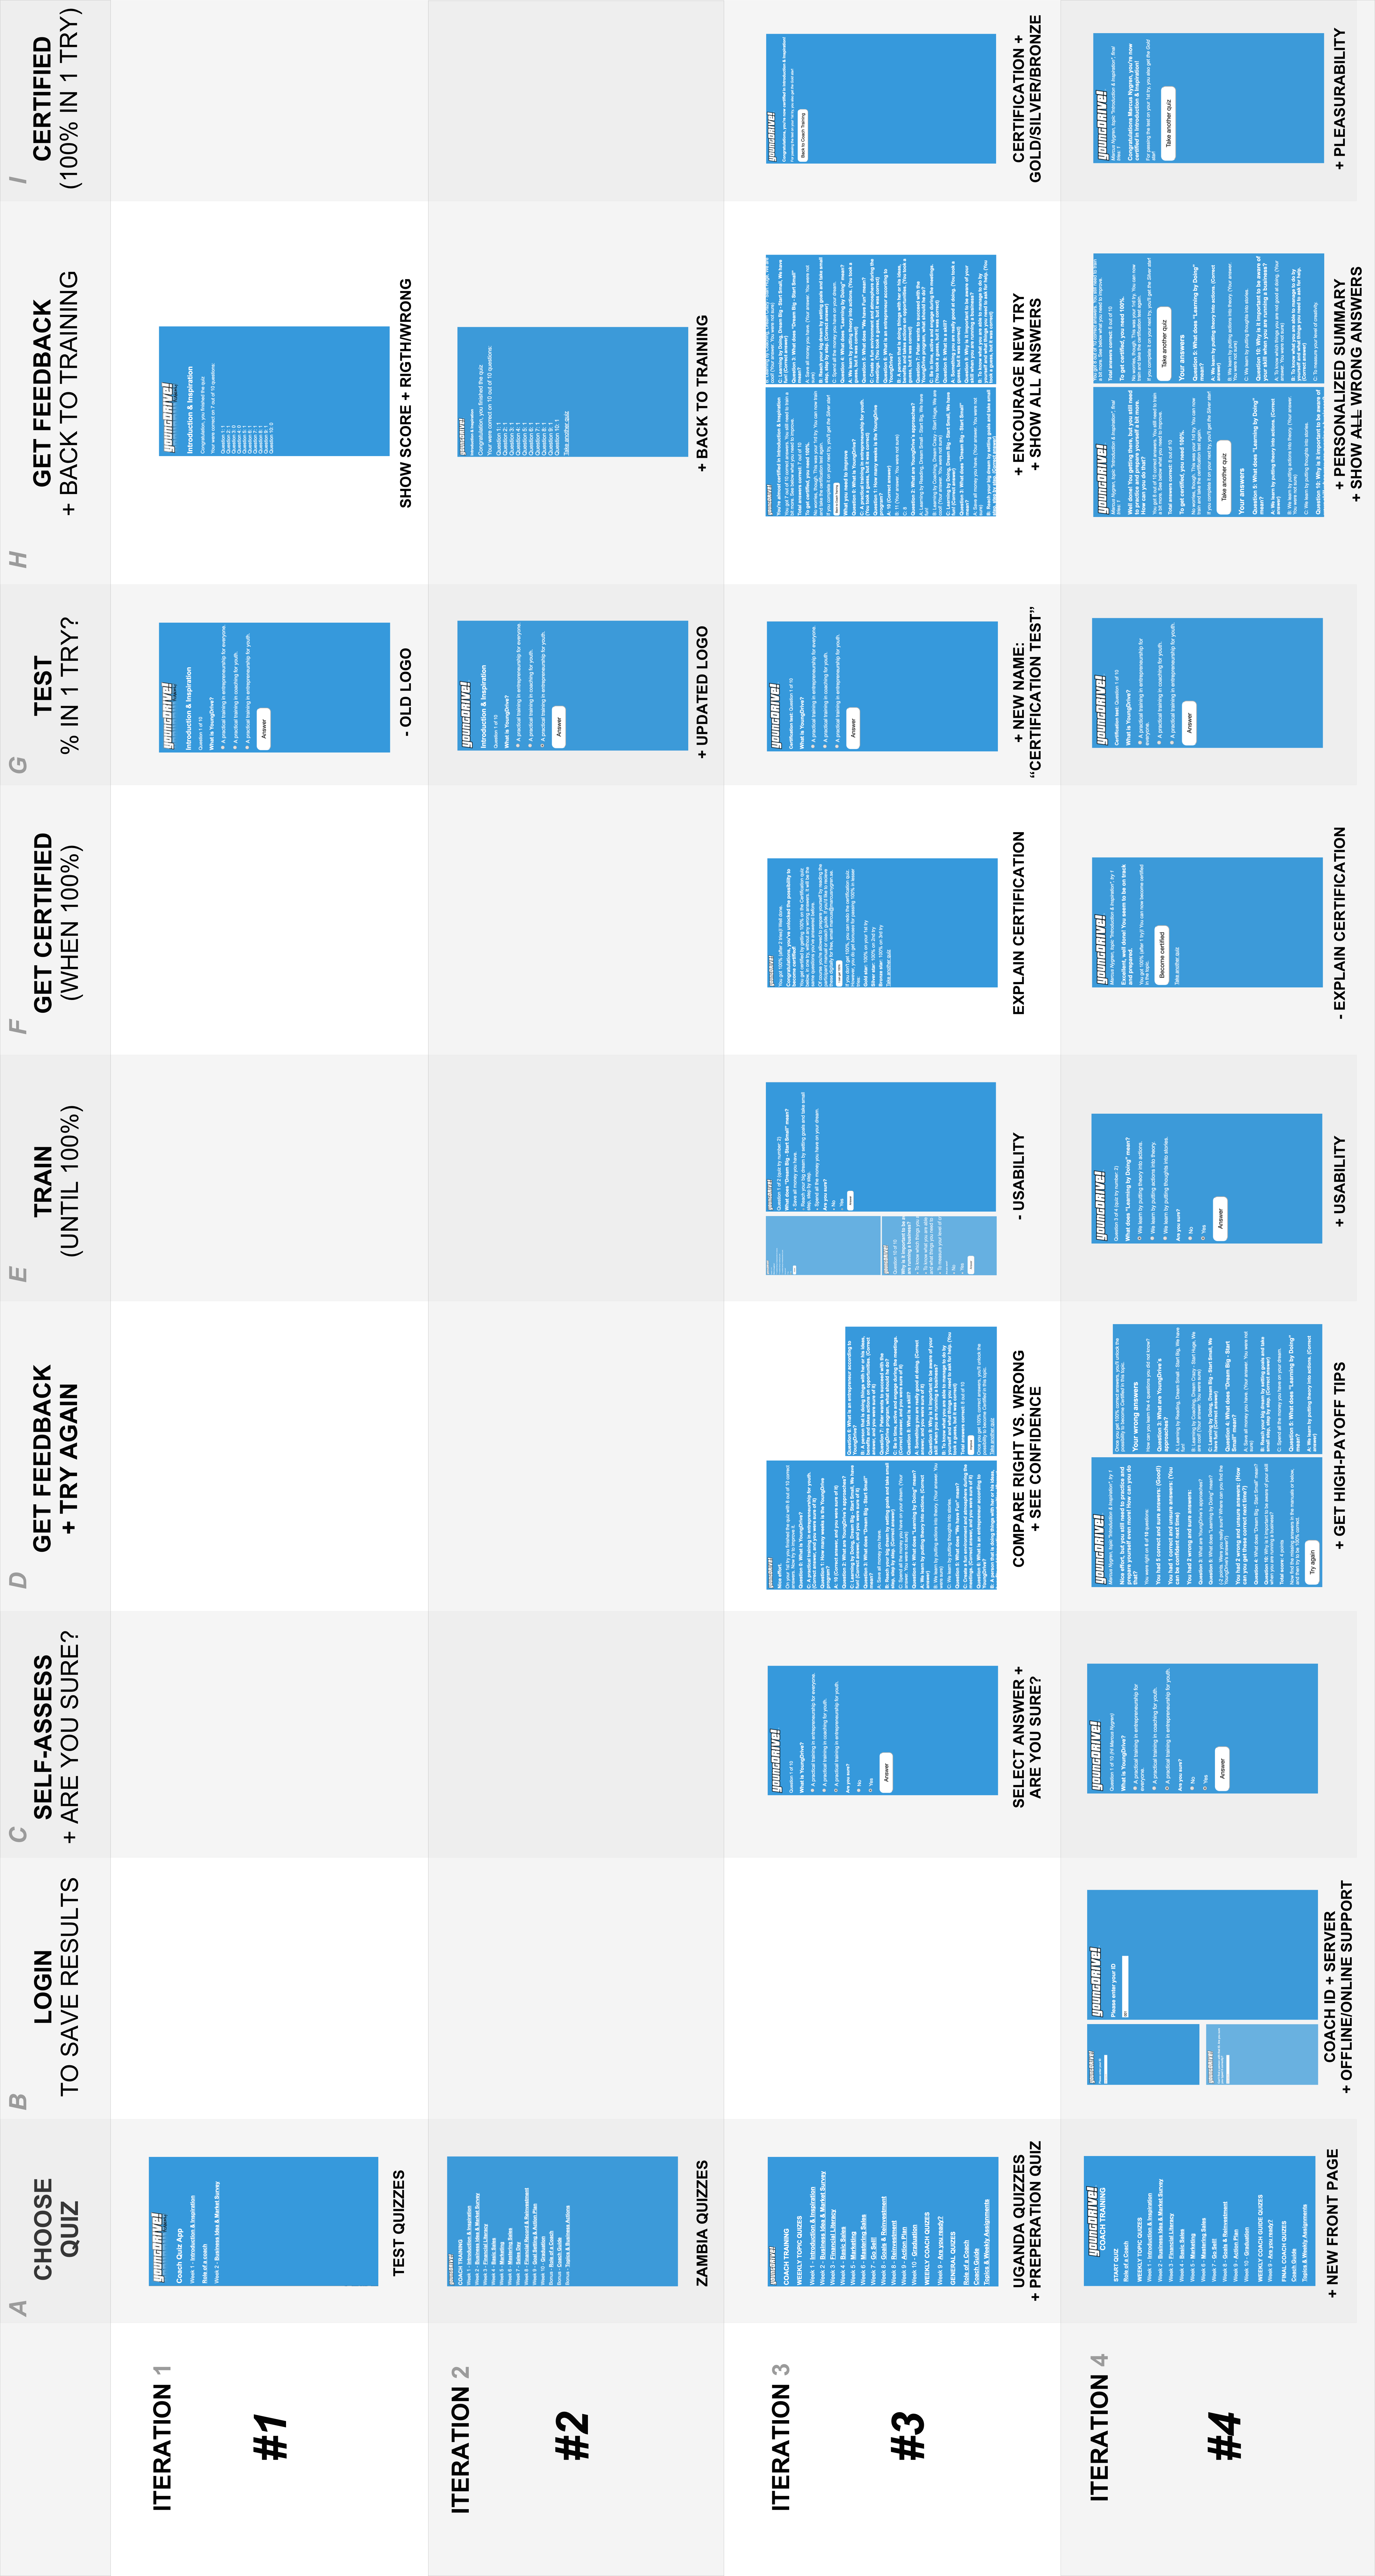
\includegraphics[width=1.0\textwidth]{IterationMapLowRes.png}
    \caption{The app flow described as a timeline (A-I), per iteration (1-4). E.g. in iteration 4, login (B4) appears after choosing quiz to take (A4).}
    \label{fig:iteration-map}
  \end{figure}

  %\subsection{Iteration \#1}

  There was no developed application at this point.


  The quiz flow iteration 1-2 was a standard multiple-choice quiz game, designed for assessment, but not for learning. In a scoreboard, they could see which questions they were awarded points for and not, with a total score. In the end of iteration 2, whey were encouraged to go back to the start screen, to redo the same quiz again, or select a new one.

  %\subsection{Iteration \#2}

  \subsubsection{Result}
  Quiz-flödet 1.0: standard multiple-choice, designat för assessment, men ej för learning
  Besvara multiple-choice-frågor
  Få resultat-tavla med Question 1: 0, Question 2: 1, samt "Total score: X/X"
  Gå tillbaka till startskärm

  \subsection{Iteration 3}

  \subsubsection{Result}
  Quiz-flöde 2.0: designat för learning och självreflektion, men ej för effektivitet
  vid varje fråga besvarar du det alternativ du tror är rätt samt "Are you sure?" Yes/No
  vid färdigt quiz, få en resultattavla med personliserad feedback
  läsa igenom dina felaktiga svar och hur säker du varit på dem
  observerat de korrekta svaren
  klicka "Improve" för att bara få dina felaktiga svar igen
  upprepa tills inga felaktiga svar var kvar (det står "quiz try: 3", om det är försök 3)
  vid 100%, låsa upp "I can get 100%" (som är hela quizet igen)
  innan dess, uppmuntrades du läsa igenom coach/deltagar-manualen
  om du då fick något fel, fick du gå tillbaka till träning igen
  om alla rätt på, blev du Certified coach. Om du klarade det på första försöket, fick du även en guldstjärna (andra försöket = silver, tredje försöket = brons)
  sedan kunde du ta ett annat quiz
  Kommentar, fördelar med feedback-läge:
  Genom att på varje fråga besvara "Are you sure?": Yes/No, så stärker vi inte bara coachens meta-kognitiva förmåga, utan vi kan vi även ge personliserad feedback i resultattavlan, istället för att bara visa Question 1: 1 point. Question 2: 0 points, som i Iteration 2.

  Detta gör att coachen kan reflektera över sitt lärande på t.ex. följande sätt:
  - få en självförtroende-boost (via feedback "You were correct, and you were sure")
  - gå från gissning till självsäkerhet (via feedback "You guessed, but you were correct")
  - ändra uppfattning snabbare (via feedback "You were incorrect, but you were sure")
  - uppmuntra coachen att läsa i manualen (via feedback "You were incorrect, and you were not sure")

  Fördelar med tränings-läge, och certifikations-läge:
  Jag gillar idén att när coachen har kunnat svara rätt på alla frågor, kunna befästa kunskapen med hjälp av certifikations-läget, då coachen ska kunna få 100\% rätt på 1 försök.

  \subsection{Iteration \#4}

  %Result

  \todo{Show images of final app - on mobile, tablet and desktop?}


\section{Iteration 1}

Here the results from the qualitative and quantative data for iteration 1 are shown, together with conclusions.

\subsection{Qualitative data}

\subsubsection{Entrepreneurship education considerations}
Throught early interviews with YoungDrive staff, it is clear that YoungDrive's entrepreneurship education methodology goes hand in hand with the presented theory. It's mottos are: "Dream big, start small", "Learning by doing" and "We have fun!" \citep{youngdrive}.

Both in regards to designing for the users and for the above reason, the app should be a complement to YoundDrive's existing training material and the structure of the program.

A challenging part of the work is that YoungDrive consists of both the practical skills of the entrepreneur, theoretical material of running a business, and an entrepreneurial mindset. Therefore, both how to assess knowledge, and build habits, needs to be examined.

\subsubsection{Understanding the coach situation}

A CBT can be responsible for from 7 up to 12 different youth groups in different programs, and such a high number places huge demands on the CBT.

Even if there are only 7 groups, being behind on schedule or not being confident, can be very demanding.

\textbf{Stayover at Patrick:} På morgonen visade Patrick mig hur han jobbar med deras tomt, var det odlas ris, och andra råvaror, deras djur, deras story från Syd-Sudan, till Kampala, till hyddan här i Tororo, och hans värderingar.

Efter en ungdomssession nästföljande dag besökte vi och hälsade kort på en av de 2 CBT:s vi har session med idag. Sedan hade jag och Patrick den obligatoriska review av ungdoms-sessionen, och jag bjöd honom på middag. Kl. 19 ringde hans fru (som har börjat få tecken av malaria) och skyndade hem.

Nästa ungdomssession fick jag besöka en annan CBT. Vi var tidiga. Sedan började jag prata med henne, och fick bra tillfälle att intervjua henne och även förklara för henne vad jag gjorde där. Det blev underligt att förklara för henne: Patrick påminde, när jag tabbat mig, att “Marcus, du måste förklara för X vad en app är”. Så hon fick låna min mobil, och jag förklarade att app var kort för applikation, och att för varje applikation har ett eget syfte, t.ex. ta foton. Jag bad henne klicka, svårt, råkade klicka åt henne, men sedan lät jag henne göra. Efter hon sett att det hon såg i skärmen var det hon såg på riktigt, blev hon jätteglad och började fundera vad hon skulle fota. Hon reste sig och gick runt hörnet, och jag följde efter. Hon fotade, efter att noggrannt tänkt igenom, att hon fotade buskarna med frukt. Sedan sade jag hon kunde fortsätta fota, och då tog hon ett litet runt hus utanför.


\subsubsection{Different kind of coaches}

The interviews with CBTs, PLs and stakeholders led to the realization that different coaches handles this differently well.

Depending on the situation, e.g. you are not confident, or you are falling behind with the schedule, you can be in one of these need groups.

\begin{itemize}
  \item The ideal coach
  \item The realistic coach
  \item The challenged coach
\end{itemize}

It was discovered, that coach confidence comes largely from being able to have good youth sessions.

\subsubsection{A good youth session}

For having a good youth session, these are the most important attributes:

\begin{itemize}
  \item Correct information
  \item Correct structure
  \item Time management
  \item Fun atmosphere
\end{itemize}

The fact that the coach knows they have these qualities, leads to self confidence from the coach. This in turn, leads to better meetings with the youth.

\subsubsection{The room for a digital solution}

It is definitely a problem that so extremely few have smartphones.

This needs to be designed for. Either, I build only for the use case of having an app tailored for the coach training, where the donated devices can be used.

Alternatively, I design only for the users that does have a smartphone, and count that more will get smartphones in the future.

Thirdly, I can use a SMS tool, not building an app but an SMS-based service, which also could be an app. Such tools exists, and are compatible with multiple-choice questions, like VOTO Mobile.

\subsection{Quantative data}

    %What the data said

    Two workshops were held, which together would inform the future development of an application.

    There were the findings from those two workshops:

    \subsubsection{Workshop \#1: Customer Journey Map: A day as a coach}

    After lunch, I held two workshops with the coaches. The first one continued from where the interviews, “A day as a coach”, using a customized Customer Journey Map. First, three personas were created based on the interviews: an “ideal coach”, “realistic coach”, and “poor coach” were named. I had created a timeline with “Before”, “During [the youth sesssion]”, and “After”, and each post-it color represented one persona: John, Joan, and Suzan. They understood the timeline and personas they created very effortlessly.

    %After the 15 minute introduction, they started with 5 minutes + 10 minutes discussion mapping out Before, During, After for the ideal coach, John. Green postits were used.

    %Since it took too much time to do this for the other two personas, they were given 5 minutes to either use pink post-its for steps that a realistic coach would skip, and yellow notes that the coach would do differently. This worked well, and the results were discussed within the 5 minutes between the coaches, and explained during 5 minutes witth audio recording.

    %Since they were understandingly tired, they were given a 10 minute break, during which time they were asked to think about things that could go wrong for the sad/angry persona, Suzan. When I got back from the toilet, they had already started working! I took time of 5 minutes, and they walked through the concerns and it’s effects, just like they had did with the 2nd persona.

    The first workshop was finished with many important insights. \todo{Add image of CJM and the insights}

    \subsubsection{Workshop \#2: Quizical and Duolingo}

    Quizoid and Duolingo were tested to understand the technical possibilites of the coaches.

    The result was that the app can place itself somewhere in the middle of the two, regarding difficulty level.

    Patrick [från YoungDrive] undrade om han kunde låna en smartphone under tiden jag var här.

    Efter workshopen, berättade han:

    “Vet du vad Marcus, idag har en av mina drömmar gått i uppfyllelse.”
    Det var första gången han använde en smartphone

    Even for coaches that had never touched a smartphone before, some concepts were easily understood (like using the camera and Quizical).

    Other concepts were harder (e.g. accidently getting to the settings menu, unlocking the device, understanding Cut the Rope 2, or training languages using Duolingo with advanced interactions). Point and click is easily understood, whereas sliding is much more unnatural.

    Also, it’s important that the app is fail-safe - but how do I avoid errors with the Android OS and iOS? A lot of training is needed to avoid errors, or I need to find another solution.

\subsection{Conclusions}

\subsubsection{Motivation of app}
The scope of the app is to examine and strengthen the entrepreneurship the student already has. One important goal is to give good feedback.

\textbf{Assessment of knowledge and skills is today mostly based on how good they feel can answer the youth’s question, and how the audience reacts}
Is this a good way of assessing? I see two problems. First, the feedback comes only after a session is carried out. Second, it is a very subjective approach. Third, this feedback is not sent to Patrick and Christine, unless they’re visiting.

\textbf{Technology could increase accuracy and accountability}
Most coaches plan their next session during the morning, or immediately after a session with their group. Since a coach has somewhere between 7-10 groups (some even more), and the youth groups are at different modules, there is a lot of knowledge for the coach to handle - not only theoretical knowledge, but also the struggles of the youth, assignment presentations, workshops to be facilitated, etc.

It is easy for a coach not to do everything as planned or as specified in the manual. By an app, they could keep a record of the module content, and see when and if they do need to refresh their skills.

\textbf{The users are already motivated to become a better coach.} Thus, I can follow Sierra's advise designing for the compelling context.

My compelling context is that I want to help you become an even better coach.

The better user point of view: don’t just make a better coach training app - make a better user of coach training material.

For me, this means:

"Given a teaching situation among the youth group, a great coach can teach an entrepreneurship topic more consistent with what the coach material said."

"Given a question in the app, a great coach will get the right answer more often, and increasingly leverage the correct answer to their coach situation."

\subsubsection{Insights}

\textbf{What's it like being a coach?} \todo{Översätt till svenska}
I iteration 1 fanns ingen digital ansats alls. Jag var i Tororo för att besvara "What's it like being a coach?". Upptäckte att vad det innebär att vara en bra YoungDrive-coach, är att kunna ha bra ungdoms-sessioner. För att ha bra ungdoms-sessioner, är din självkänsla och självförtroende enormt viktigt. Och det är inte alla coacher som har detta, och därför skiljer sig kvaliteten mycket, vilket Josefina upplever som en utmaning.

Jag började leta efter hur och var en coach-app kan underlätta. En aktivitet som alla coacher har gemensamt för lärande och avgörande för coachens framgång, är (1) coach-träningen (som jag redan visste var viktig), men framför allt (2) förberedelserna av en ungdomssession. Jag övertygade Josefina att vi skulle ha ett mycket fokus på (2) än hon tänkt. Medan Josefina kan vara inblandad i (1), kan en app vara extremt viktig i (2), upptäckte jag under mina fält-besök på ungdomssessioner och intervjuer med coacher och projektledare.

Enligt Iteration 1: Självförtroende = empowerment
Enligt iteration 1 kom självförtroende ifrån att under ungdomstillfället kunna ha: Correct Information, Correct Structure, Time Management, och Fun Atmosphere. Det är alltså detta appen borde testa och träna.

For iteration 2, there were two main insights to consider from iteration \#1:

\begin{itemize}
\item The aim is for the coach to feel self-confidence for its youth session
\item The skill to be trained is having a youth session
\end{itemize}

During the evaluation meeting with Linköping University and YoungDrive, it was the determined that Iteration \#1, provided answers for research question \#1, \#2, and \#3.

The iteration had provided a good basis for answering research question \#5.


\section{Iteration 2}

Here the results from the qualitative and quantative data for iteration 2 are shown, together with conclusions.

\subsection{Iteration \#2}

According to the final interview with Josefina, she does not wish the app to replace her. She enjoys teacher, thinks she has an important role, and suggests the app to be designed to support her and the coaches, not replace her.

\subsection{Iteration \#2}

    %What the data said

    \subsubsection{Results from the coaches}

    \subsubsection{Day 2}
    Most coaches prefer tablet: 5 prefer tablet, 2 smartphone, and 2 computer.

    \subsubsection{Day 3}
    iOS no longer allows uncertified app install from computer: you need to have paid a license even for unreleased apps, being a "Trusted developer". This stops the app from being able to be installed on all the iOS devices, so that only the web version can be used.

    Thus, only the web app was tested from Wednesday and onwards.

    This was a problems, as the app regurly crashed at refresh because of low internet capacity.

    Sometimes, it was neeed to go to the other office where there was wifi, to refresh the webpage, and go back to the location. This of course would not work for Josefina.

    \subsubsection{Day 4}
    Tested using the quiz before the session.

    \subsubsection{Day 5}
    On day 5, the schedule was:

    \begin{itemize}
      \item "Goal setting" part 2
      \item App test: "Goal setting" after-quiz and "Graduation" pre-quiz.
      \item "Graduation"
    \end{itemize}

    In "Goal setting", one coach were an outlier to the other high results, scoring 9/19 answers correct.

    \subsubsection{Observable trends from the coaches}

\subsection{Iteration \#2}



\subsubsection{Bonus results: Testing the app outside the YoungDrive context}
Back in Uganda, a test was done with refugee innovators, at the Humanitarian Innovation Jam.

Also, the app was tested on a university student from Makarere University

The test with the refugee innovatiors were surprisingly intriguing and successful.

It was found that refugee innovators says they would have a great need for such an app.

The university student from Makarere University scored 100\% correct, in spite of not having any entrepreneurship training. This showed that guessing was possible, or that the quizzes were too easy.

\subsubsection{Findings}

Test with university student scored 100\% correct, means that common sense can go a long way, and that the results can't be 100\% trustworthy, and that multiple-choice questions has serious issues - this, we already knew during and before the coach training - but it needs to be taken care of

The app would be great and could actually work outside the physical coach training - with revision, be stand-alone, even being able to distribute online.

Now there are observable evidence for what the interactions from Iteration 1 showed:

\begin{itemize}
\item The purpose of the coach training should be to prepare the coach in having great youth sessions
\item Therefore, this is what the quizzess should assess
\item What it really means being a good YoungDrive coach, is having good youth sessions
\item Josefina would have liked to be able to stop coaches from having taught, if they do not have 90-100 \% correct information on the subject
\item Today, Josefina can not assess this. This means that some coaches, are teaching incorrect information to hundreds of youth.
\item Here, the quiz has a very good need to fill.
\end{itemize}

With all of these findings in summary, it can be concluded that an app for coach training, and an app to use before a youth session, could be the same app, since the purpose of preparing the coach to be great with its youth session is the same.

From the interviews, it was learned that while it \textit{may} be technically possible, the teacher desires the app support her, not replace her.


\section{Iteration 3}

Here the results from the qualitative and quantative data for iteration 1 are shown, together with conclusions.

\subsection{Iteration \#3}

  %What the observations said

  Bugs
  Simpler design than I thought (KISS)

  Using the quiz before the session increases learning, slightly decreases fun of the session, according to coaches

  Fun and encouraging

  \subsubsection{Josefina feedback}

  \textbf{Acceptance criteria}

If you have a high score, you are ready. If not, you need to redo the quiz.

If you are 8/10 or lower, you are in the red zone. If lower than 10/10, they are not ready, the motivation being that what they don't know, they will teach in an improper way: affecting hundreds of youth. This is why Josefina thinks they should need all of the answers correct.

\subsection{Iteration \#3}

    %What the data said

    \subsubsection{Results from the coaches}

    \subsubsection{Observable trends from the coaches}

\subsection{Iteration \#3}

  för learning och självreflektion, men ej för effektivitet

  \textit{Deliberate practice: not satisfied.} The lesson learned is that while the app is now designed for learning, it is not designed for speed. It took too long to get certified to be within the realms of deliberate practice.

  Help them practice right. Goal: design practice exercises that will take a fine-grained task from unreliable to 95\% reliability, within one to three 45-90-minute sessions.

  If not possible, don't continue trying: split into smaller tasks, Sierra says.

  While there was now an MVP for the coach training, there was not yet a MVP for the youth session; only an MP (minimum product, but not viable yet).

  To improve effectiveness, it was determined that "learning by thinking", regarding metacognitive skills, could be beneficial. This would help the coach to analyze and evaluate its own learning, possibly improving faster in the app.

  \subsubsection{Bonus results}
  The Kampala test showed how well the app works for learning entrepreneurship also outside of the YoungDrive context. Some modifications would greatly improve this further.


\section{Iteration 4}

Here the results from the qualitative and quantative data for iteration 4 are shown, together with conclusions.

\subsection{Iteration \#4}

Everyone now thought the app was good and easy to use.

With the Plan Tororo staff, it was shown how important the certification mode was: even though one group had 100\% on their first try, and a person had 1 wrong answer, the person with 1 wrong answer got 100\% on the certification, while the 100\% group had 1 wrong answer.

It is therefore determined, that when all of the answers can be answered correctly, after having gotten all answers correct once, that the knowledge is reliable - this is deliberate practice.

\subsection{Iteration \#4}

    %What the data said

    \subsubsection{Results from the coaches}

    \todo{Add table from Google Sheets}

    \subsubsection{Data observations}

% Important to be objective
% En diskussion om hur resultaten kan användas i praktiken är också i de flesta fall belysande och relevant i rapporter

% https://liu.se/ias/kontakta-oss?l=en

In this section, the conclusions from the different group characteristics are presented.

Early observations from the pre-test data was that a surprising number of cells were left blank. One user had not done the pre-test, where some had left questions unanswered (most commonly "Do you own a company?" (should have used the word "business"), plus "Hours of preperation" and "Occations for a youth session" (there is a tendency this might be because they were not proud of their answers, because of correlations with low quiz results).

Missing cells was not as obvious with the app results, were users could not progress in a quiz without answering both the question and the confidence. However, none of the passed quiz 9 certification answers had been submitted. Thus, it was needed to add these from the manual recordings, which had been used as a backup in case anything like this would happen.


There were a number of quick insights that could be drawn before the parallell coordinates visualization: there was a surprisingly low number of answers where the user answered the question without confidence. Also, more users had started a quiz without finishing it than anticipated. Finally, a lot of users had done quizes that were not Topic quiz 3 and Coach quiz 9, which might indicate high interest (if they did more than 2 quizes) or confusion (if they did not do 3 or 9, but they did do other quizes) during the app evaluation. This meant that on some aspects, there were less data than anticipated, (which was troublesome, as there were already few data points), and some aspects where there was more data than anticipated (that were overlooked).

First-hand insights before the parallell coordinates were that there was a strong corrolation between pre-quiz results and quiz 9 try 1 (slightly visible also in quiz 3 try 1, but with more outliers). Also, with manuals there was a higher probability to finishing quiz 9 training + certification.

\subsubsection{Statistical analysis}
Statistical analysis unfortunately showed that none of the results were statistically significant to be notable using linear regression, or any of the other statistical methods detailed in the methodical framework.

\subsubsection{Parallel coordinates visualization}
The interactive parallel coordinates visualization could give many more insights, more faster than the static presentations in Google Sheets.

\textbf{Youth mentor (brun), 6 st vs. CBT (blå), 14 st}
* Youth mentors has higher school level than CBT's
* 1/6 Youth mentors had brought manual, compared with 8/14 CBT's
* Only 1 CBT has above 2 (1 st 3) on School, while YM have (2st 0, 1 2st, 2 2st)
* Inverse correlation: CBT old, YM young
* There are no female Youth Mentors (i.e. 100\% male Youth Mentors)
* All of the YM's run their own businesses, compared with 5/10 for CBT's
* Only CBT's said they didn't feel comfortable with smartphone (2 st) - because of age?
* Seemingly no difference CBT vs. YM in when prepares for session
* All YM prepares 2 times for session, while CBT can train also 3 or 1 time)
* 13/14 CBT's gjorde quiz 3 try 1, 6/6 YM's
* YM's och CBT's presterar lika på quiz 3 try 1
* CBT 6/14 st certifierade, YM 4/6 st

Quiz 9 (rött=CBT:
* 6 CBT's gör ej Q9 try 1, 2 YM gör ej
* YM är top performers på Q9 try 1 jämfört med CBT's
* endast 1 YM klarade däremot träningen, medan

* YM's är bättre på quiz 9 try 1 än CBT's
* Det är endast 1/7 som klarade quiz 9 training som är Youth Mentor
* Antal försök man gjorde är likvärdigt, förutom en YM som hade 12 försök (och klarade quiz)
* Det var endast 2 st som klarade certifieringen, och båda dessa var YM och kvinnliga

\textbf{Women}

It is clear from the data that women:
* Have lower education level than the men
* Spread results on the pre-test (probably because of school level)
* Half of them are around 25 years old, half spread out (up until 45 years old)
* 2/6 har eget företag
* Det är bara 1 som ej preppar alls
* 1 st som endast preppar 1 gång, alla andra preppar 2 gånger (3 st) eller 3 gånger (2 st)
* Alla hade max 1 fel på quiz 3 på första försöket!
* De som ej hade rätt, tog det bara 2:a (1 person) eller 3:e försöket (1 person)

* 3/6 gjorde certifieringen - kolla upp: började de?

* Alla förutom 1 tjej gjorde svåraste quizet. De hade minst 42\%! Varav 2 st hade 67\%, 1 hade 50, 1 hade 42, och 1 hade 83

* Quiz 9 tjejerna hade mycket högre lägstanivå () än killarna (, och mycket högre högstanivå än killarna () - tiden är jämförbar, med svag tendens snabbare tjejer
* Av de som hade 50\% på 1:a försöket, gick det betydligt snabbare för tjejerna än killarna att jobba igenom quizet - tyder på att tjejerna är säkrare på materialet än tjejerna - dessutom är det bara 2 killar som fick över 50\% på första försöket
* Om du kollar tvärtom, så är det bara 1 tjej som fick under 50\% på första försöket, medan det var 8 killar
* Quiz 3 syns ej lika tydlig skillnad (OBS: kolla vilken fråga de flesta hade fel på, och kolla om det skiljer sig mellan killar och tjejer)
* Skolnivå verkar oberende på hur quizen blir, om man kollar quiz 9
* Tjejer, antal försök quiz 9 hade de 2 (2 st), 5 (2st, 12 (1st) försök innan de klarade - bland killarna var det 5 (1st) och 7 (1st). Men sedan så var det 0 av killarna som blev certified, men 2 tjejer (de som gjorde på 12 försök och 2 försäk). Att antal försök skiljde sig mellan 2 och 12, men ändå klarar det, berättar att antal försök kanske ej korrelerar. Den på 12 försök hade 70\% på försök, och jobbade igen de 12 försöken väldigt snabbt.
* Den andra tjejen som klarade certifikation quiz 9 klarade 83\% försök 1, (hade tillgång till hjälp), klarade träningen sedan på 2 försök.

Slutsats:
* Anställ bara tjejer. De har högre kunskap och förbereder sig mer, trots lägre skolutbildning.

\textbf{Use of participant and coach manuals}

Användande av appen:
* Vi hittade ingen korrelation quiz-resultat 9 första försöket om man fick hjälp eller inte, antagligen pga att man ej använder manualen före

\textbf{Certified quiz 9}
Only two people were fast enough to get certified on the final quiz before the app evaluation ended.

Characteristics were:
* Both of them used the manual
* Both of them were CBT's, not youth mentors
* Both were women
* They were 24 or 26 years old
* They had a good pre-test score (57\% or 71\%)
* They had top scores (1st place and 2nd place (shared with one other)) on quiz 9 try 1
* They had high scores on quiz 3 try 1 (100\% and 92\%
* They prepared many times per youth session (2 or 3 times)

What didn't seem to matter:
* Number of tries quiz 9 (12 vs 2 on Q9)
* Time to pass training quiz 9 (35.5, slowest vs 12 minutes, below average)
* When day trained (1 trained same day, 1 trained the day before)
* One had a business, one didn't
* School level (1 S?, one S lower)

Other:
* They were medium skilled on using a smartphone


\subsection{Iteration \#4}

\todo{Add everything from the mindmap}


%\section{Qualitative Data}
%
%  Here the results from the qualitative data for iteration 1, 2, %3 and 4 are shown.
%
%  \subsection{Qualitative data}

\subsubsection{Entrepreneurship education considerations}
Throught early interviews with YoungDrive staff, it is clear that YoungDrive's entrepreneurship education methodology goes hand in hand with the presented theory. It's mottos are: "Dream big, start small", "Learning by doing" and "We have fun!" \citep{youngdrive}.

Both in regards to designing for the users and for the above reason, the app should be a complement to YoundDrive's existing training material and the structure of the program.

A challenging part of the work is that YoungDrive consists of both the practical skills of the entrepreneur, theoretical material of running a business, and an entrepreneurial mindset. Therefore, both how to assess knowledge, and build habits, needs to be examined.

\subsubsection{Understanding the coach situation}

A CBT can be responsible for from 7 up to 12 different youth groups in different programs, and such a high number places huge demands on the CBT.

Even if there are only 7 groups, being behind on schedule or not being confident, can be very demanding.

\textbf{Stayover at Patrick:} På morgonen visade Patrick mig hur han jobbar med deras tomt, var det odlas ris, och andra råvaror, deras djur, deras story från Syd-Sudan, till Kampala, till hyddan här i Tororo, och hans värderingar.

Efter en ungdomssession nästföljande dag besökte vi och hälsade kort på en av de 2 CBT:s vi har session med idag. Sedan hade jag och Patrick den obligatoriska review av ungdoms-sessionen, och jag bjöd honom på middag. Kl. 19 ringde hans fru (som har börjat få tecken av malaria) och skyndade hem.

Nästa ungdomssession fick jag besöka en annan CBT. Vi var tidiga. Sedan började jag prata med henne, och fick bra tillfälle att intervjua henne och även förklara för henne vad jag gjorde där. Det blev underligt att förklara för henne: Patrick påminde, när jag tabbat mig, att “Marcus, du måste förklara för X vad en app är”. Så hon fick låna min mobil, och jag förklarade att app var kort för applikation, och att för varje applikation har ett eget syfte, t.ex. ta foton. Jag bad henne klicka, svårt, råkade klicka åt henne, men sedan lät jag henne göra. Efter hon sett att det hon såg i skärmen var det hon såg på riktigt, blev hon jätteglad och började fundera vad hon skulle fota. Hon reste sig och gick runt hörnet, och jag följde efter. Hon fotade, efter att noggrannt tänkt igenom, att hon fotade buskarna med frukt. Sedan sade jag hon kunde fortsätta fota, och då tog hon ett litet runt hus utanför.


\subsubsection{Different kind of coaches}

The interviews with CBTs, PLs and stakeholders led to the realization that different coaches handles this differently well.

Depending on the situation, e.g. you are not confident, or you are falling behind with the schedule, you can be in one of these need groups.

\begin{itemize}
  \item The ideal coach
  \item The realistic coach
  \item The challenged coach
\end{itemize}

It was discovered, that coach confidence comes largely from being able to have good youth sessions.

\subsubsection{A good youth session}

For having a good youth session, these are the most important attributes:

\begin{itemize}
  \item Correct information
  \item Correct structure
  \item Time management
  \item Fun atmosphere
\end{itemize}

The fact that the coach knows they have these qualities, leads to self confidence from the coach. This in turn, leads to better meetings with the youth.

\subsubsection{The room for a digital solution}

It is definitely a problem that so extremely few have smartphones.

This needs to be designed for. Either, I build only for the use case of having an app tailored for the coach training, where the donated devices can be used.

Alternatively, I design only for the users that does have a smartphone, and count that more will get smartphones in the future.

Thirdly, I can use a SMS tool, not building an app but an SMS-based service, which also could be an app. Such tools exists, and are compatible with multiple-choice questions, like VOTO Mobile.

%  \subsection{Iteration \#2}

According to the final interview with Josefina, she does not wish the app to replace her. She enjoys teacher, thinks she has an important role, and suggests the app to be designed to support her and the coaches, not replace her.

%  \subsection{Iteration \#3}

  %What the observations said

  Bugs
  Simpler design than I thought (KISS)

  Using the quiz before the session increases learning, slightly decreases fun of the session, according to coaches

  Fun and encouraging

  \subsubsection{Josefina feedback}

  \textbf{Acceptance criteria}

If you have a high score, you are ready. If not, you need to redo the quiz.

If you are 8/10 or lower, you are in the red zone. If lower than 10/10, they are not ready, the motivation being that what they don't know, they will teach in an improper way: affecting hundreds of youth. This is why Josefina thinks they should need all of the answers correct.

%  \subsection{Iteration \#4}

Everyone now thought the app was good and easy to use.

With the Plan Tororo staff, it was shown how important the certification mode was: even though one group had 100\% on their first try, and a person had 1 wrong answer, the person with 1 wrong answer got 100\% on the certification, while the 100\% group had 1 wrong answer.

It is therefore determined, that when all of the answers can be answered correctly, after having gotten all answers correct once, that the knowledge is reliable - this is deliberate practice.

%
%\section{Quantitative Data}
%
%  Here the results from the quantitative data for iteration 1, 2, %3 and 4 are shown.
%
%  \subsection{Quantative data}

    %What the data said

    Two workshops were held, which together would inform the future development of an application.

    There were the findings from those two workshops:

    \subsubsection{Workshop \#1: Customer Journey Map: A day as a coach}

    After lunch, I held two workshops with the coaches. The first one continued from where the interviews, “A day as a coach”, using a customized Customer Journey Map. First, three personas were created based on the interviews: an “ideal coach”, “realistic coach”, and “poor coach” were named. I had created a timeline with “Before”, “During [the youth sesssion]”, and “After”, and each post-it color represented one persona: John, Joan, and Suzan. They understood the timeline and personas they created very effortlessly.

    %After the 15 minute introduction, they started with 5 minutes + 10 minutes discussion mapping out Before, During, After for the ideal coach, John. Green postits were used.

    %Since it took too much time to do this for the other two personas, they were given 5 minutes to either use pink post-its for steps that a realistic coach would skip, and yellow notes that the coach would do differently. This worked well, and the results were discussed within the 5 minutes between the coaches, and explained during 5 minutes witth audio recording.

    %Since they were understandingly tired, they were given a 10 minute break, during which time they were asked to think about things that could go wrong for the sad/angry persona, Suzan. When I got back from the toilet, they had already started working! I took time of 5 minutes, and they walked through the concerns and it’s effects, just like they had did with the 2nd persona.

    The first workshop was finished with many important insights. \todo{Add image of CJM and the insights}

    \subsubsection{Workshop \#2: Quizical and Duolingo}

    Quizoid and Duolingo were tested to understand the technical possibilites of the coaches.

    The result was that the app can place itself somewhere in the middle of the two, regarding difficulty level.

    Patrick [från YoungDrive] undrade om han kunde låna en smartphone under tiden jag var här.

    Efter workshopen, berättade han:

    “Vet du vad Marcus, idag har en av mina drömmar gått i uppfyllelse.”
    Det var första gången han använde en smartphone

    Even for coaches that had never touched a smartphone before, some concepts were easily understood (like using the camera and Quizical).

    Other concepts were harder (e.g. accidently getting to the settings menu, unlocking the device, understanding Cut the Rope 2, or training languages using Duolingo with advanced interactions). Point and click is easily understood, whereas sliding is much more unnatural.

    Also, it’s important that the app is fail-safe - but how do I avoid errors with the Android OS and iOS? A lot of training is needed to avoid errors, or I need to find another solution.

%  \subsection{Iteration \#2}

    %What the data said

    \subsubsection{Results from the coaches}

    \subsubsection{Day 2}
    Most coaches prefer tablet: 5 prefer tablet, 2 smartphone, and 2 computer.

    \subsubsection{Day 3}
    iOS no longer allows uncertified app install from computer: you need to have paid a license even for unreleased apps, being a "Trusted developer". This stops the app from being able to be installed on all the iOS devices, so that only the web version can be used.

    Thus, only the web app was tested from Wednesday and onwards.

    This was a problems, as the app regurly crashed at refresh because of low internet capacity.

    Sometimes, it was neeed to go to the other office where there was wifi, to refresh the webpage, and go back to the location. This of course would not work for Josefina.

    \subsubsection{Day 4}
    Tested using the quiz before the session.

    \subsubsection{Day 5}
    On day 5, the schedule was:

    \begin{itemize}
      \item "Goal setting" part 2
      \item App test: "Goal setting" after-quiz and "Graduation" pre-quiz.
      \item "Graduation"
    \end{itemize}

    In "Goal setting", one coach were an outlier to the other high results, scoring 9/19 answers correct.

    \subsubsection{Observable trends from the coaches}

%  \subsection{Iteration \#3}

    %What the data said

    \subsubsection{Results from the coaches}

    \subsubsection{Observable trends from the coaches}

%  \subsection{Iteration \#4}

    %What the data said

    \subsubsection{Results from the coaches}

    \todo{Add table from Google Sheets}

    \subsubsection{Data observations}

% Important to be objective
% En diskussion om hur resultaten kan användas i praktiken är också i de flesta fall belysande och relevant i rapporter

% https://liu.se/ias/kontakta-oss?l=en

In this section, the conclusions from the different group characteristics are presented.

Early observations from the pre-test data was that a surprising number of cells were left blank. One user had not done the pre-test, where some had left questions unanswered (most commonly "Do you own a company?" (should have used the word "business"), plus "Hours of preperation" and "Occations for a youth session" (there is a tendency this might be because they were not proud of their answers, because of correlations with low quiz results).

Missing cells was not as obvious with the app results, were users could not progress in a quiz without answering both the question and the confidence. However, none of the passed quiz 9 certification answers had been submitted. Thus, it was needed to add these from the manual recordings, which had been used as a backup in case anything like this would happen.


There were a number of quick insights that could be drawn before the parallell coordinates visualization: there was a surprisingly low number of answers where the user answered the question without confidence. Also, more users had started a quiz without finishing it than anticipated. Finally, a lot of users had done quizes that were not Topic quiz 3 and Coach quiz 9, which might indicate high interest (if they did more than 2 quizes) or confusion (if they did not do 3 or 9, but they did do other quizes) during the app evaluation. This meant that on some aspects, there were less data than anticipated, (which was troublesome, as there were already few data points), and some aspects where there was more data than anticipated (that were overlooked).

First-hand insights before the parallell coordinates were that there was a strong corrolation between pre-quiz results and quiz 9 try 1 (slightly visible also in quiz 3 try 1, but with more outliers). Also, with manuals there was a higher probability to finishing quiz 9 training + certification.

\subsubsection{Statistical analysis}
Statistical analysis unfortunately showed that none of the results were statistically significant to be notable using linear regression, or any of the other statistical methods detailed in the methodical framework.

\subsubsection{Parallel coordinates visualization}
The interactive parallel coordinates visualization could give many more insights, more faster than the static presentations in Google Sheets.

\textbf{Youth mentor (brun), 6 st vs. CBT (blå), 14 st}
* Youth mentors has higher school level than CBT's
* 1/6 Youth mentors had brought manual, compared with 8/14 CBT's
* Only 1 CBT has above 2 (1 st 3) on School, while YM have (2st 0, 1 2st, 2 2st)
* Inverse correlation: CBT old, YM young
* There are no female Youth Mentors (i.e. 100\% male Youth Mentors)
* All of the YM's run their own businesses, compared with 5/10 for CBT's
* Only CBT's said they didn't feel comfortable with smartphone (2 st) - because of age?
* Seemingly no difference CBT vs. YM in when prepares for session
* All YM prepares 2 times for session, while CBT can train also 3 or 1 time)
* 13/14 CBT's gjorde quiz 3 try 1, 6/6 YM's
* YM's och CBT's presterar lika på quiz 3 try 1
* CBT 6/14 st certifierade, YM 4/6 st

Quiz 9 (rött=CBT:
* 6 CBT's gör ej Q9 try 1, 2 YM gör ej
* YM är top performers på Q9 try 1 jämfört med CBT's
* endast 1 YM klarade däremot träningen, medan

* YM's är bättre på quiz 9 try 1 än CBT's
* Det är endast 1/7 som klarade quiz 9 training som är Youth Mentor
* Antal försök man gjorde är likvärdigt, förutom en YM som hade 12 försök (och klarade quiz)
* Det var endast 2 st som klarade certifieringen, och båda dessa var YM och kvinnliga

\textbf{Women}

It is clear from the data that women:
* Have lower education level than the men
* Spread results on the pre-test (probably because of school level)
* Half of them are around 25 years old, half spread out (up until 45 years old)
* 2/6 har eget företag
* Det är bara 1 som ej preppar alls
* 1 st som endast preppar 1 gång, alla andra preppar 2 gånger (3 st) eller 3 gånger (2 st)
* Alla hade max 1 fel på quiz 3 på första försöket!
* De som ej hade rätt, tog det bara 2:a (1 person) eller 3:e försöket (1 person)

* 3/6 gjorde certifieringen - kolla upp: började de?

* Alla förutom 1 tjej gjorde svåraste quizet. De hade minst 42\%! Varav 2 st hade 67\%, 1 hade 50, 1 hade 42, och 1 hade 83

* Quiz 9 tjejerna hade mycket högre lägstanivå () än killarna (, och mycket högre högstanivå än killarna () - tiden är jämförbar, med svag tendens snabbare tjejer
* Av de som hade 50\% på 1:a försöket, gick det betydligt snabbare för tjejerna än killarna att jobba igenom quizet - tyder på att tjejerna är säkrare på materialet än tjejerna - dessutom är det bara 2 killar som fick över 50\% på första försöket
* Om du kollar tvärtom, så är det bara 1 tjej som fick under 50\% på första försöket, medan det var 8 killar
* Quiz 3 syns ej lika tydlig skillnad (OBS: kolla vilken fråga de flesta hade fel på, och kolla om det skiljer sig mellan killar och tjejer)
* Skolnivå verkar oberende på hur quizen blir, om man kollar quiz 9
* Tjejer, antal försök quiz 9 hade de 2 (2 st), 5 (2st, 12 (1st) försök innan de klarade - bland killarna var det 5 (1st) och 7 (1st). Men sedan så var det 0 av killarna som blev certified, men 2 tjejer (de som gjorde på 12 försök och 2 försäk). Att antal försök skiljde sig mellan 2 och 12, men ändå klarar det, berättar att antal försök kanske ej korrelerar. Den på 12 försök hade 70\% på försök, och jobbade igen de 12 försöken väldigt snabbt.
* Den andra tjejen som klarade certifikation quiz 9 klarade 83\% försök 1, (hade tillgång till hjälp), klarade träningen sedan på 2 försök.

Slutsats:
* Anställ bara tjejer. De har högre kunskap och förbereder sig mer, trots lägre skolutbildning.

\textbf{Use of participant and coach manuals}

Användande av appen:
* Vi hittade ingen korrelation quiz-resultat 9 första försöket om man fick hjälp eller inte, antagligen pga att man ej använder manualen före

\textbf{Certified quiz 9}
Only two people were fast enough to get certified on the final quiz before the app evaluation ended.

Characteristics were:
* Both of them used the manual
* Both of them were CBT's, not youth mentors
* Both were women
* They were 24 or 26 years old
* They had a good pre-test score (57\% or 71\%)
* They had top scores (1st place and 2nd place (shared with one other)) on quiz 9 try 1
* They had high scores on quiz 3 try 1 (100\% and 92\%
* They prepared many times per youth session (2 or 3 times)

What didn't seem to matter:
* Number of tries quiz 9 (12 vs 2 on Q9)
* Time to pass training quiz 9 (35.5, slowest vs 12 minutes, below average)
* When day trained (1 trained same day, 1 trained the day before)
* One had a business, one didn't
* School level (1 S?, one S lower)

Other:
* They were medium skilled on using a smartphone


%
%\section{Insights}
%
%  \subsection{Conclusions}

\subsubsection{Motivation of app}
The scope of the app is to examine and strengthen the entrepreneurship the student already has. One important goal is to give good feedback.

\textbf{Assessment of knowledge and skills is today mostly based on how good they feel can answer the youth’s question, and how the audience reacts}
Is this a good way of assessing? I see two problems. First, the feedback comes only after a session is carried out. Second, it is a very subjective approach. Third, this feedback is not sent to Patrick and Christine, unless they’re visiting.

\textbf{Technology could increase accuracy and accountability}
Most coaches plan their next session during the morning, or immediately after a session with their group. Since a coach has somewhere between 7-10 groups (some even more), and the youth groups are at different modules, there is a lot of knowledge for the coach to handle - not only theoretical knowledge, but also the struggles of the youth, assignment presentations, workshops to be facilitated, etc.

It is easy for a coach not to do everything as planned or as specified in the manual. By an app, they could keep a record of the module content, and see when and if they do need to refresh their skills.

\textbf{The users are already motivated to become a better coach.} Thus, I can follow Sierra's advise designing for the compelling context.

My compelling context is that I want to help you become an even better coach.

The better user point of view: don’t just make a better coach training app - make a better user of coach training material.

For me, this means:

"Given a teaching situation among the youth group, a great coach can teach an entrepreneurship topic more consistent with what the coach material said."

"Given a question in the app, a great coach will get the right answer more often, and increasingly leverage the correct answer to their coach situation."

\subsubsection{Insights}

\textbf{What's it like being a coach?} \todo{Översätt till svenska}
I iteration 1 fanns ingen digital ansats alls. Jag var i Tororo för att besvara "What's it like being a coach?". Upptäckte att vad det innebär att vara en bra YoungDrive-coach, är att kunna ha bra ungdoms-sessioner. För att ha bra ungdoms-sessioner, är din självkänsla och självförtroende enormt viktigt. Och det är inte alla coacher som har detta, och därför skiljer sig kvaliteten mycket, vilket Josefina upplever som en utmaning.

Jag började leta efter hur och var en coach-app kan underlätta. En aktivitet som alla coacher har gemensamt för lärande och avgörande för coachens framgång, är (1) coach-träningen (som jag redan visste var viktig), men framför allt (2) förberedelserna av en ungdomssession. Jag övertygade Josefina att vi skulle ha ett mycket fokus på (2) än hon tänkt. Medan Josefina kan vara inblandad i (1), kan en app vara extremt viktig i (2), upptäckte jag under mina fält-besök på ungdomssessioner och intervjuer med coacher och projektledare.

Enligt Iteration 1: Självförtroende = empowerment
Enligt iteration 1 kom självförtroende ifrån att under ungdomstillfället kunna ha: Correct Information, Correct Structure, Time Management, och Fun Atmosphere. Det är alltså detta appen borde testa och träna.

For iteration 2, there were two main insights to consider from iteration \#1:

\begin{itemize}
\item The aim is for the coach to feel self-confidence for its youth session
\item The skill to be trained is having a youth session
\end{itemize}

During the evaluation meeting with Linköping University and YoungDrive, it was the determined that Iteration \#1, provided answers for research question \#1, \#2, and \#3.

The iteration had provided a good basis for answering research question \#5.

%  \subsection{Iteration \#2}



\subsubsection{Bonus results: Testing the app outside the YoungDrive context}
Back in Uganda, a test was done with refugee innovators, at the Humanitarian Innovation Jam.

Also, the app was tested on a university student from Makarere University

The test with the refugee innovatiors were surprisingly intriguing and successful.

It was found that refugee innovators says they would have a great need for such an app.

The university student from Makarere University scored 100\% correct, in spite of not having any entrepreneurship training. This showed that guessing was possible, or that the quizzes were too easy.

\subsubsection{Findings}

Test with university student scored 100\% correct, means that common sense can go a long way, and that the results can't be 100\% trustworthy, and that multiple-choice questions has serious issues - this, we already knew during and before the coach training - but it needs to be taken care of

The app would be great and could actually work outside the physical coach training - with revision, be stand-alone, even being able to distribute online.

Now there are observable evidence for what the interactions from Iteration 1 showed:

\begin{itemize}
\item The purpose of the coach training should be to prepare the coach in having great youth sessions
\item Therefore, this is what the quizzess should assess
\item What it really means being a good YoungDrive coach, is having good youth sessions
\item Josefina would have liked to be able to stop coaches from having taught, if they do not have 90-100 \% correct information on the subject
\item Today, Josefina can not assess this. This means that some coaches, are teaching incorrect information to hundreds of youth.
\item Here, the quiz has a very good need to fill.
\end{itemize}

With all of these findings in summary, it can be concluded that an app for coach training, and an app to use before a youth session, could be the same app, since the purpose of preparing the coach to be great with its youth session is the same.

From the interviews, it was learned that while it \textit{may} be technically possible, the teacher desires the app support her, not replace her.

%  \subsection{Iteration \#3}

  för learning och självreflektion, men ej för effektivitet

  \textit{Deliberate practice: not satisfied.} The lesson learned is that while the app is now designed for learning, it is not designed for speed. It took too long to get certified to be within the realms of deliberate practice.

  Help them practice right. Goal: design practice exercises that will take a fine-grained task from unreliable to 95\% reliability, within one to three 45-90-minute sessions.

  If not possible, don't continue trying: split into smaller tasks, Sierra says.

  While there was now an MVP for the coach training, there was not yet a MVP for the youth session; only an MP (minimum product, but not viable yet).

  To improve effectiveness, it was determined that "learning by thinking", regarding metacognitive skills, could be beneficial. This would help the coach to analyze and evaluate its own learning, possibly improving faster in the app.

  \subsubsection{Bonus results}
  The Kampala test showed how well the app works for learning entrepreneurship also outside of the YoungDrive context. Some modifications would greatly improve this further.

%  \subsection{Iteration \#4}

\todo{Add everything from the mindmap}


%\begin{chapter-appendix}

%\section{Proof-Appendix}
%
Det här är en appendix-del av det aktuella kapitlet.

%\end{chapter-appendix}
